\documentclass[11pt,a4paper]{article}

\usepackage[utf8]{inputenc}
\usepackage[english]{babel}
\usepackage[T1]{fontenc}

\usepackage{amsmath,amssymb,amsfonts}

\usepackage{hyperref}
\usepackage{graphicx}

\title{Statistical Methods for Machine Learning - Exam}
\author{Sebastian Paaske Tørholm}

\begin{document}
\maketitle

\section{General comments}
The code is written in MATLAB R2012b, and makes use of the built-in library
functions. I've chosen to do this due to the implementation being robust
and easy to use.

\section{Sunspot Prediction}
For question 1, I have chosen to use a maximum likelihood estimate, with a
linear design matrix. I do not use a built-in implementation.

The maximum likelihood model found is defined by the following weight vector:

\[
    \mathbf{w}_{ML} = \begin{pmatrix} 10.844 \\ -0.062 \\ 0.121 \\ -0.012 \\ -0.570 \\ 1.284 \end{pmatrix}
\]


For question 2, I use MATLAB's built in neural network implementation for
this. I've chosen to use a feed-forward neural network with 5, 10 and 15
hidden neurons. The network is trained using the RProp algorithm described at
the lectures.

The implementation makes use of regularization and early stopping to improve
the generalization performance and help reduce overfitting.

\begin{figure}[h!]
    \centering
    \begin{tabular}{|l|l|l|}
        \hline
        Model & RMS (training data) & RMS (testing data) \\
        \hline
        Linear ML & 14.067 & 18.770 \\
        NN (5 hidden neurons) & 13.390 & 19.695 \\
        NN (10 hidden neurons) & 13.210 & 21.924 \\
        NN (15 hidden neurons) & 12.902 & 24.196 \\ 
        \hline
    \end{tabular}
    \caption{RMS of the sunspot predictions.}
    \label{sunspots-rms}
\end{figure}

In \autoref{sunspots-rms}, we see that the neural networks provide a better
prediction on the training data, but that the linear model wins on the testing
data. This could be due to the neural network overfitting itself to the
training data, and we in fact see that the fewer neurons we use, the better
the RMS is on the testing data.

One could suspect that given the good performance on the linear model, a model
with shortcuts may provide a better performance for the neural network, as it
could introduce more linearity.

\begin{figure}[h!]
    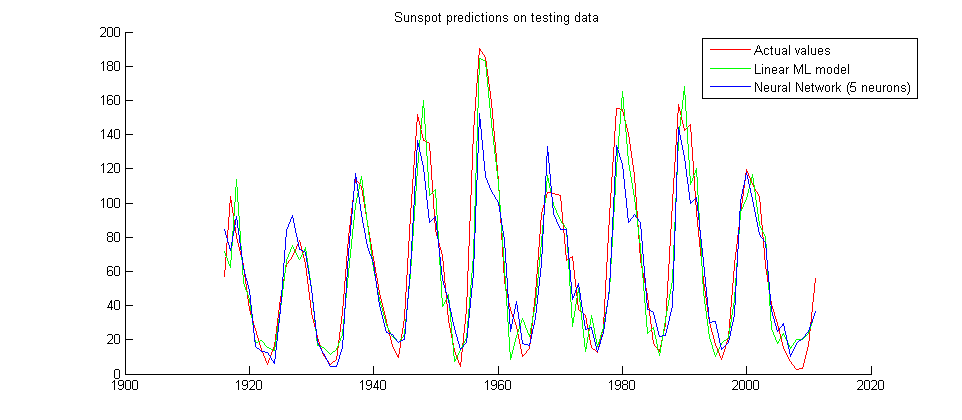
\includegraphics[width=\textwidth]{images/sunspots-testing.png}

    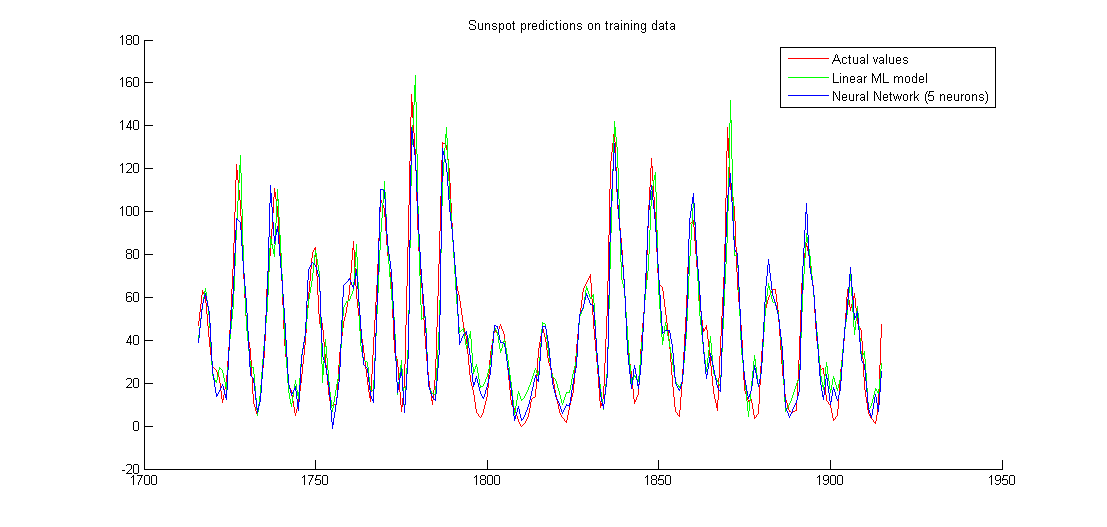
\includegraphics[width=\textwidth]{images/sunspots-training.png}
    \caption{Plots of the predictions on the sunspot testing and training data.}
    \label{sunspots-plots}
\end{figure}

In \autoref{sunspots-plots} we see the predictions plotted against the actual
expected number of sunspots. The linear model does seem to follow the data
more closely, explaining the lower RMS. Especially around 1960, the large
number of sunspots isn't sufficiently modelled by the NN model, whereas the
linear model captures it.

\section{Surveying the sky}
$\sigma_{\text{Jaakkola}}$ was computed by dividing the dataset into stars
and quasars, followed by finding the median as described. This gives
$\sigma_{\text{Jaakkola}} = 3.907$.

For the grid search, I've chosen to use $b = e$ as the base number. Instead of
computing $\gamma_{\text{Jaakkola}}$, I make use of

\[
    \sigma_{\text{Jaakkola}} \cdot b^{-i/2} = \sqrt{1/(2 \gamma_{\text{Jaakkola}} b^i)}
\]

I use the built-in SVM functionality for MATLAB as my SVM implementation. The
data for the SVM is automatically normalized by the implementation, improving
SVM performance, as we saw in assignment 3.

The grid search yielded

\[ \sigma = \sigma_{\text{Jakkola}} \cdot e^{-3/2} = 0.872 \quad\quad C = e^3 = 20.086 \]

as optimal hyperparameters. Using these hyperparameters yields the 0-1 correct rates shown in
\autoref{star-correctrates}. 

\begin{figure}[h!]
    \centering
    \begin{tabular}{|l|l|}
        \hline
        Data set & 0-1 correct rate \\
        \hline
        Training set & $98.64\%$ \\
        Testing set  & $97.87\%$ \\
        \hline
    \end{tabular}
    \caption{0-1 correct rates for the SVM with optimal hyperparameters.}
    \label{star-correctrates}
\end{figure}

\section{Overfitting}
\begin{description}
    \item[Traditional overfitting] {
        On the sunspot prediction, we could see that increasing the number of
        hidden nodes in the neural network gave an increase in the RMS on the
        testing set. If one furthermore didn't employ countermeasures like
        early stopping, the effect of this would be more pronounced.

        Likewise, performing a different segmentation, giving a too small test
        set may induce overfitting.
    }
    \item[Parameter tweak overfitting] {
        We performed our model selection in question 4 based solely on the
        training set performance. If we were to take the test set into
        consideration, we effectively train the model based on both the
        training and test set, leaving us no measure of its effectiveness.
    }
    \item[Brittle measure] {
        Instead of determining the optimal hyperparameters for our SVM using
        $k$-fold crossvalidation, we could have used an approach more prone
        to overfitting, such as leave-one-out crossvalidation. This method is
        more poorly suited for measuring performance, as the fact that we're
        validatidating against only one sample each iteration allows outliers
        to affect the results more negatively.
    }
    \item[Bad statistics] {
        The datasets do not directly present any obvious pitfalls with
        regards to statistical analyses. Naturally, one should always be
        careful when dealing with statistics, however, and make sure that all
        pre-requisites and assumptions are in fact well founded.
    }
    \item[Choice of measure] {
        When working with a data set, one will often measure the results in
        several different ways, to try to get a feel for how well the methods
        one's employing works. This is a good thing, if the entire suite of
        results is passed on. However, it's often tempting to only report the
        results that look good, giving a potentially misleading picture of the
        algorithm effectiveness.
    }
    \item[Incomplete Prediction] {
        Since we're not dealing with multiclass predictions, this is not as
        applicable to these datasets.
    }
    \item[Human-loop overfitting] {
        When working with the datasets, one could easily be tempted to try
        many different methods, and see how well they perform on the test
        set. Observing poor performance can lead to wanting to try different
        approaches, using performance on the test set as a measure. This could
        lead to over-fitting the method to the test set.
    }
    \item[Data set selection] {
        Unless you're developing new methods, the problem of data set selection
        does not apply. If you're simply trying to apply machine learning
        techniques to a specific dataset, then the data set is select for you.
    }
    \item[Reprobleming] {
        Looking at the graph of the training data in \autoref{sunspots-plots},
        we see that the interval from approximately 1790 to 1840 has an
        extraordinarily low number of sunspots. One could imagine someone
        trying to remove those years from the training data to attempt to
        improve classification.
    }
    \item[Old datasets] {
        Again, unless you're developing new methods, using old data sets
        isn't a problem. If you're developing a new method, you should make
        sure to test the method on a variety of data sets, both new and old,
        and report performance on all data sets you test on. This will help
        determine if the method itself is over-fitted to the specific dataset.

        If working on a specific problem, having a method that is over-fitted
        to that specific problem isn't a big issue, as generalized performance
        is less important than the algorithm working well on the problem it's
        being used on.
    }
\end{description}

\section{Wheat Seeds}

For question 6, the principal components analysis is performed using the
MATLAB built-in \texttt{princomp} function. If we look at the eigenvalue
spectrum in \autoref{eigenvalue-spectrum}, we see that in the unnormalized
data, the first and second principal components capture most of the variance
in the data. Looking a the normalized data, we see that the third principal
component brings a significant portion as well. Therefore, if we wish to
reduce the data to two dimensions, we should perform our dimensional reduction
using the results of the PCA on the unnormalized data.

\begin{figure}[h!]
    \centering
    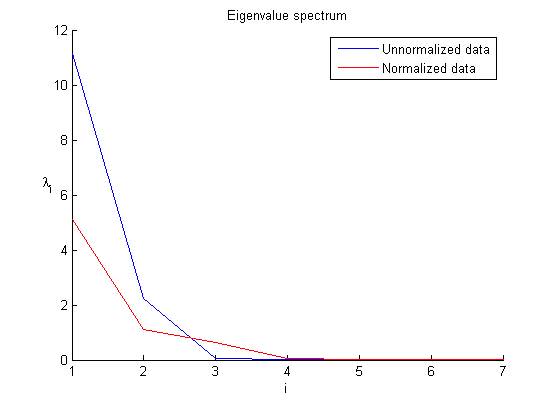
\includegraphics[width=0.7\textwidth]{images/eigenvalue-spectrum}
    \caption{Eigenvalue spectrum on unnormalized and normalized data.}
    \label{eigenvalue-spectrum}
\end{figure}

The result of projecting the data onto the two first principal components
found in the PCA can be seen in \autoref{seeds-projected}. We observe a nice
separation of the different classes in the data.

\begin{figure}[h!]
    \centering
    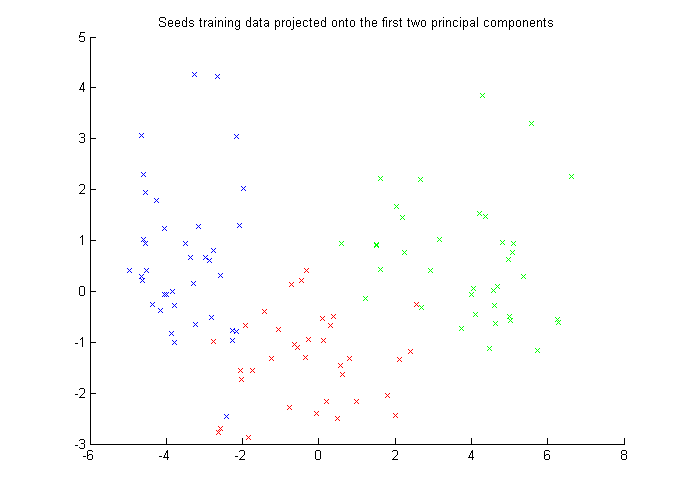
\includegraphics[width=0.7\textwidth]{images/seeds-projected}
    \caption{The seed training data projected onto its first two principal components.}
    \label{seeds-projected}
\end{figure}

For question 7, I use MATLAB's built in implementation of $k$-means
clustering. In \autoref{seeds-kmeans}, we see the results of the clustering.
We can observe that the clusters match up with the expected classification
quite well, with the exception of a slight bit of misclassification at the
boundaries between two classes. The centroids look very reasonable.

\begin{figure}[h!]
    \centering
    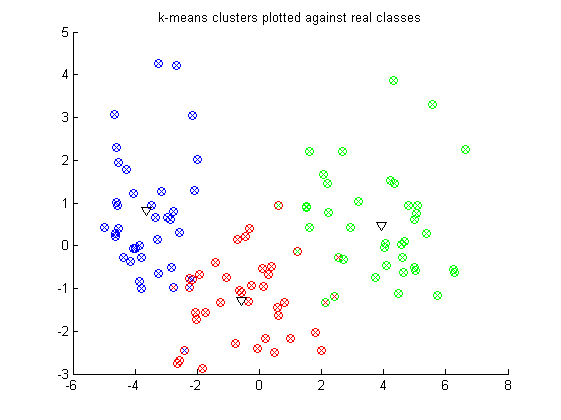
\includegraphics[width=0.7\textwidth]{images/seeds-kmeans}
    \caption{The projected seed training data plotted with (1) crosses being
        the real classification, (2) circles being the classification found by
        $k$-means, (3) the black triangles being the cluster centroids.}
    \label{seeds-kmeans}
\end{figure}

For question 8, I use the suggested $k$-nearest neighbor for non-linear
classification and LDA for linear classification.

The $k$-nearest neighbor uses MATLAB's built in implementation. The
classification is attempted for $k = 3, 5, 7, 9, 15$. The success rates are
listed in \autoref{seeds-knn-success}. We see that $k = 3$ and $k = 15$ work
slightly better than the rest, but all in all the differences aren't too
large. This is further seen in \autoref{seeds-knn-plot}, where $k=3$ and $k=7$
can be compared. No matter the $k$, the same points remain problematic, mainly
around the edges of the groups.

\begin{figure}[h!]
    \centering
    \begin{tabular}{|l|l|}
        \hline
        $k$ & 0-1 correct rate \\
        \hline
        3  & 86\% \\ 
        5  & 85\% \\
        7  & 84\% \\
        9  & 84\% \\
        15 & 86\% \\
        \hline
    \end{tabular}
    \caption{0-1 correct rates for $k$-NN classification, for differerent $k$.}
    \label{seeds-knn-success}
\end{figure}

\begin{figure}[h!]
    \centering
    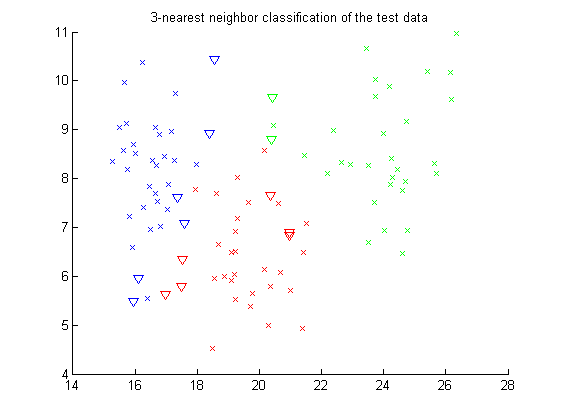
\includegraphics[width=.45\textwidth]{images/seeds-3nn-success}
    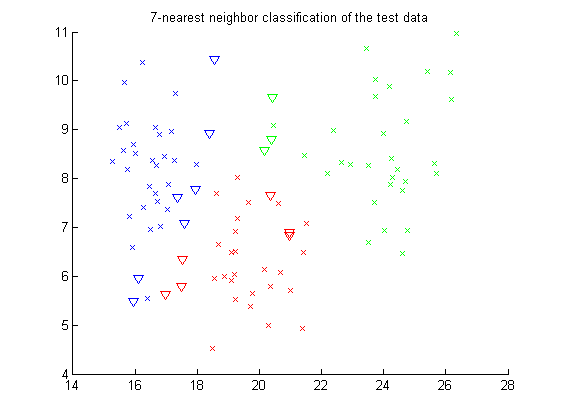
\includegraphics[width=.45\textwidth]{images/seeds-7nn-success}
    \caption{The results of $3$-NN and $7$-NN classification. The crosses are
             correctly classified points, and the triangles are misclassified.}
    \label{seeds-knn-success}
\end{figure}

For LDA, I use MATLAB's built-in linear classification. In
\autoref{seeds-lda-train} we see the results of applying the LDA to the
training set, where it achieves a $99\%$ success rate, misclassifying only a
single point. This indicates that it has learned the training set quite well.
Using the same model on the test data, as seen in \autoref{seeds-lda-test},
gives a $94\%$ success rate, giving a significant improvement as opposed to
the best $k$-NN classification.

\begin{figure}[h!]
    \centering
    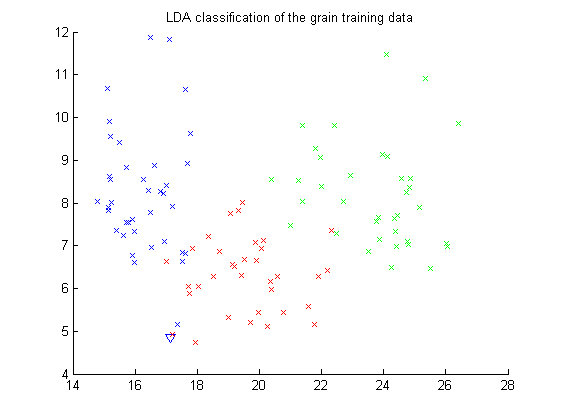
\includegraphics[width=.75\textwidth]{images/seeds-lda-train}
    \caption{The classification provided by LDA on the training set. Crosses are correctly classified points, triangles misclassified.}
    \label{seeds-lda-train}
\end{figure}

\begin{figure}[h!]
    \centering
    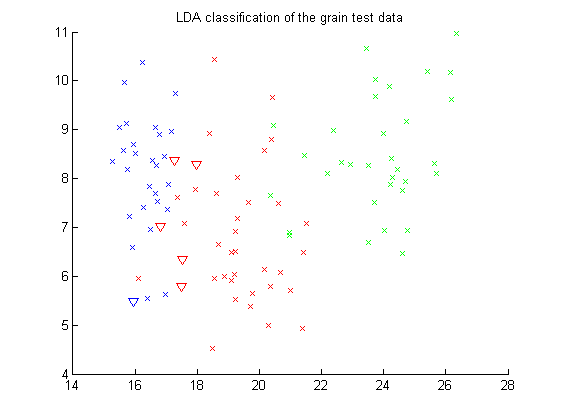
\includegraphics[width=.75\textwidth]{images/seeds-lda-test}
    \caption{The classification provided by LDA on the testing set. Crosses are correctly classified points, triangles misclassified.}
    \label{seeds-lda-test}
\end{figure}

\end{document}

